% !TeX program = xelatex
% UTF-8. Measured figures use experiments/figures/*.pdf; table values come from
% experiments/results/tables/*.tex (generated by experiments/report_assets.py).
% Other figures and references are embedded. No BibTeX or shell-escape is required.
% Sections flow continuously; final pagination depends on fonts.
\documentclass[a4paper,11pt]{article}
\usepackage[margin=22mm]{geometry}
\usepackage{kotex}
\usepackage{amsmath,amssymb,mathtools,bm}
\usepackage{graphicx,xcolor,booktabs,array,tabularx}
\usepackage{enumitem}
\usepackage{tikz,pgfplots}
\usetikzlibrary{arrows.meta,positioning,calc}
\pgfplotsset{compat=1.18}
\usepackage[font=small,labelfont=bf,hypcap=false]{caption}
\usepackage[authoryear,round]{natbib}
\usepackage{hyperref}
\usepackage{seqsplit}

\hypersetup{colorlinks=true,linkcolor=blue!50!black,
  citecolor=blue!50!black,urlcolor=blue!50!black,
  pdftitle={EM의 Convergence Guarantee 및 GMM Learning}}
% #1: 표시할 절 번호의 label, #2: 이동할 위치, #3: 번호 뒤에 붙는 구절.
% 번호와 구절이 한 링크가 되어 PDF에서 클릭하면 #2로 이동한다.
\DeclareRobustCommand{\seclink}[3]{\hyperref[#2]{\ref*{#1}#3}\hspace{0pt}}
\DeclareRobustCommand{\secref}[2]{\seclink{#1}{#1}{#2}}
\definecolor{mainblue}{HTML}{215A8A}
\definecolor{mainorange}{HTML}{C36624}
\definecolor{maingreen}{HTML}{287D68}
\newcommand{\E}{\mathbb{E}}
\newcommand{\R}{\mathbb{R}}
\newcommand{\KL}{\operatorname{KL}}
\newcommand{\Normal}{\mathcal{N}}
\newcommand{\diag}{\operatorname{diag}}
\newcommand{\softmax}{\operatorname{softmax}}
\newcommand{\poly}{\operatorname{poly}}
\newcommand{\tr}{\operatorname{tr}}
\newcommand{\given}{\,\middle|\,}
\newcolumntype{Y}{>{\raggedright\arraybackslash}X}
\makeatletter\newcommand{\inputrows}[1]{\@@input #1 }\makeatother % generated table rows
\setlength{\parindent}{0pt}
\setlength{\parskip}{5pt plus 1pt}
\setlength{\emergencystretch}{2em}
\setlist{nosep,leftmargin=1.5em,topsep=4pt}
\linespread{1.06}
\numberwithin{equation}{section}
\pgfplotsset{reportaxis/.style={
  axis lines=left, tick label style={font=\scriptsize},
  label style={font=\small}, title style={font=\small},
  legend style={font=\scriptsize,draw=none,fill=white},
  grid=major,grid style={gray!15}, clip=true}}
\tikzset{box/.style={draw=mainblue,rounded corners=2pt,
  fill=mainblue!5,align=center,font=\small,inner sep=6pt},
  arrow/.style={-{Stealth[length=2mm]},thick}}
\begin{document}
\begin{center}
  {\LARGE\bfseries EM 알고리즘과 GMM 파라미터 추정방법론}\par
  \vspace{0.35em} 2024404060 강민혁
\end{center}
\section{EM 알고리즘의 Convergence Guarantee}
\subsection{Convergence Guarantee 원리}
GMM은 관측값 $x_1,\ldots,x_n\in\R^d$의 분포를 $K$개의 Gaussian component로 모형화한다.
EM은 다음 log-likelihood를 높이도록 parameter $\theta=\{\pi_k,\mu_k,\Sigma_k\}_{k=1}^{K}$를 갱신한다.
\begin{equation}
 \ell(\theta)=\sum_{i=1}^{n}\log
 \underbrace{\sum_{k=1}^{K}\pi_k\,\Normal(x_i;\mu_k,\Sigma_k)}_{p_\theta(x_i)}
 \label{eq:loglik}
\end{equation}
$\pi_k$, $\mu_k$, $\Sigma_k$는 각각 mixing coefficient, mean, covariance이며,
$\ell$은 학습 데이터에 대한 모델의 적합도를 나타낸다.

log 안에 합이 있어 $\ell$을 직접 최대화하는 해는 일반적으로 closed form으로 구할 수 없다.
EM은 관측되지 않은 component label $z_i$의 확률을 계산하고 이를 가중치로 parameter를 추정한다.
E-step은 현재 $\theta^{(t)}$에서 label의 posterior인 responsibility를 계산한다.
\begin{equation}
 r_{ik}^{(t)}=p(z_i=k\mid x_i,\theta^{(t)})
 =\frac{\pi_k^{(t)}\,\Normal(x_i;\mu_k^{(t)},\Sigma_k^{(t)})}
 {\sum_{j=1}^{K}\pi_j^{(t)}\,\Normal(x_i;\mu_j^{(t)},\Sigma_j^{(t)})}
 \label{eq:estep}
\end{equation}
이는 각 샘플을 여러 component에 확률적으로 배정하는 soft assignment이다.

M-step은 responsibility를 고정하고 가중 통계량으로 parameter를 갱신한다.
\begin{equation}
\begin{gathered}
 N_k=\sum_{i=1}^{n}r_{ik}^{(t)},\qquad
 \pi_k^{(t+1)}=\frac{N_k}{n},\qquad
 \mu_k^{(t+1)}=\frac{1}{N_k}\sum_{i=1}^{n}r_{ik}^{(t)}x_i,\\
 \Sigma_k^{(t+1)}=\frac{1}{N_k}\sum_{i=1}^{n}r_{ik}^{(t)}
 \bigl(x_i-\mu_k^{(t+1)}\bigr)\bigl(x_i-\mu_k^{(t+1)}\bigr)^{\top}
\end{gathered}
\label{eq:mstep}
\end{equation}
이 식은 complete-data log-likelihood의 조건부 기댓값
$Q(\theta\mid\theta^{(t)})=\sum_{i,k}r_{ik}^{(t)}\log\bigl(\pi_k\Normal(x_i;\mu_k,\Sigma_k)\bigr)$를
최대화하는 해이다.

이때, label의 분포 $q$에 대해 ELBO를
$\mathcal F(q,\theta)=\E_q[\log p_\theta(X,Z)]-\E_q[\log q(Z)]$로 정의하면,
다음 분해가 성립한다~\citep{dempster1977}.
\begin{equation}
 \ell(\theta)=\mathcal F(q,\theta)+\KL\bigl(q\,\|\,p_\theta(Z\mid X)\bigr)
 \label{eq:decomp}
\end{equation}
KL은 항상 0 이상이기에 $\mathcal F$는 $\ell$의 lower bound이다.
E-step에서 $q^{(t)}=p_{\theta^{(t)}}(Z\mid X)$로 두면 KL이 0이 된다.
M-step에서는 $q^{(t)}$를 고정하기에 entropy 항이 상수가 되고, $Q$를 최대화하면 $\mathcal F$도 최대화된다.
이를 바탕으로, 아래 부등식을 통해 monotonicity를 얻을 수 있다.
\begin{equation}
 \ell(\theta^{(t+1)})
 \ \overset{\text{(a)}}{\geq}\ \mathcal F(q^{(t)},\theta^{(t+1)})
 \ \overset{\text{(b)}}{\geq}\ \mathcal F(q^{(t)},\theta^{(t)})
 \ \overset{\text{(c)}}{=}\ \ell(\theta^{(t)})
 \label{eq:monotonicity}
\end{equation}
\begin{samepage}
즉 $\ell$의 증가량은 bound 증가량과 갱신 후 KL의 합으로, 둘 다 0 이상이며,
다음 E-step은 새 위치에서 다시 $\ell$에 닿는 bound를 만든다.
\end{samepage}

\begin{center}
\begin{tikzpicture}
\begin{axis}[reportaxis,width=.86\linewidth,height=5.5cm,
  xmin=0,xmax=3.4,ymin=.25,ymax=3.15,xtick={.8,1.536842},
  xticklabels={$\theta^{(t)}$,$\theta^{(t+1)}$},ytick=\empty,
  xlabel={Parameter direction (schematic)},ylabel={Objective},
  legend pos=south east]
\addplot[mainblue,very thick,domain=0:3.4,samples=100]
 {2.9-.35*(x-2.8)^2};
\addlegendentry{$\ell(\theta)$}
\addplot[mainorange,thick,domain=0:2.9,samples=100]
 {2.9-.35*(x-2.8)^2-.6*(x-.8)^2};
\addlegendentry{$\mathcal F(q^{(t)},\theta)$}
\addplot[maingreen,dashed,thick,domain=.1:3.15,samples=100]
 {2.9-.35*(x-2.8)^2-.6*(x-1.536842)^2};
\addlegendentry{$\mathcal F(q^{(t+1)},\theta)$}
\addplot[only marks,mark=*,black] coordinates
 {(.8,1.5) (1.536842,2.015789) (1.536842,2.341551)};
\draw[arrow,mainorange] (axis cs:.83,1.52)--(axis cs:1.49,1.99);
\draw[arrow,maingreen] (axis cs:1.536842,2.04)--(axis cs:1.536842,2.31);
\node[font=\scriptsize,anchor=north west] at (axis cs:.84,1.45) {(c) E-step: $\mathcal F=\ell$};
\node[font=\scriptsize,anchor=east] at (axis cs:.94,1.93) {(b) M-step};
\node[font=\scriptsize,anchor=west] at (axis cs:1.64,2.15) {(a) KL 차이};
\end{axis}
\end{tikzpicture}
\captionof{figure}{Lower-bound ascent의 개념도. (c) E-step 직후 bound는 $\theta^{(t)}$에서 $\ell$에 닿고,
(b) M-step은 bound의 꼭대기로 이동하며, (a) 새 위치에서 $\ell$은 bound보다 KL만큼 높다.
초록색 점선은 다음 E-step이 만드는 bound이다.}
\label{fig:elbo}
\end{center}

\subsection{Log-likelihood 수렴의 의미}
\label{sec:loglik}
$\ell_t=\ell(\theta^{(t)})$라 하면 식~\eqref{eq:monotonicity}에 의해
$\ell_0,\ell_1,\ldots$은 감소하지 않는다. 여기에 $\ell_t$가 발산하지 않는다는 조건이 더해지면
monotone convergence theorem에 의해 $\ell_t$는 유한한 값 $\ell_\infty$로 수렴하고,
반복 간 증가량 $\ell_{t+1}-\ell_t$는 0으로 간다.
이는 학습 데이터에 대한 objective가 일정한 값에 가까워진다는 뜻일 뿐이다.
*반복으로 그 값에 도달한다는 뜻이 아니다.
따라서, 실제로는 일반적인 early stop처럼 $\ell$의 상대 증가량이 작아지면 반복을 멈춘다.
물론, 단순히 학습이 느리게 진행되기 때문에 수렴이 느린 것일 수도 있기에, 
parameter의 변화와 수치적 안정성도 함께 확인해야 한다.
과제에서 요구하지는 않았지만, 공부하다보니 재밌어서 추가로 진행한 실험을 기술한 \seclink{sec:extension}{sec:conv-record}{절에서는}, 이 종료 기준을 만족한 뒤에도 반복을 계속하자 $\ell$이 크게 달라진 경우를 보인다.

objective가 수렴하더라도 parameter $\theta^{(t)}$가 한 점으로 수렴한다는 보장은 없다.
서로 다른 parameter가 같은 density를 나타내거나 likelihood가 평평한 구간이 있을 수
있기 때문이다. 적당한 조건에서, EM이 도달하는 점이 likelihood의 gradient가
0인 stationary point임이 알려져 있다~\citep{wu1983}.
물론, 이것이 stationary point는 global maximum을 뜻하지 않으며,
local maximum이나 saddle point일 수도 있기에 섣불리 판단함에는 주의가 필요하다.

parameter에 제약이 없으면 likelihood가 무한히 커질 수 있기에 GMM에서는 likelihood가 위로 발산하지 않는다는 조건도 확인해야 한다.
$K\geq2$에서 한 component의 mean을 관측값 $x_1$에 놓고 covariance를 $s^2I_d$로 줄이면,
식~\eqref{eq:loglik}에서 그 component의 density $\Normal(x_1;\mu_1,\Sigma_1)$은 $s^{-d}$에 비례하여 커진다. 해당 $\pi_1>0$을 고정하고 나머지 component가 다른 관측값에 양의 density를 유지하게 하면, $s\to0$에서 $p_\theta(x_1)$과 $\ell(\theta)$가 무한대로 발산하게 된다.
물론, 모든 EM이 발산함을 뜻하지는 않는다. 다만, 제약이 없는 GMM에서는
monotonicity만으로 목적함수값이 유한한 값에 수렴한다고 보장이 어렵다.
반면, 모든 covariance의 고유값에 양의 하한 $\lambda_0$를 두면
각 gaussian density의 최댓값이 $(2\pi\lambda_0)^{-d/2}$ 이하가 되기에
mixture density와 $\ell(\theta)$도 발산하지 않게 된다.
이때는 해당 제약을 만족하는 M-step을 사용해야 한다.
prior를 도입해 MAP 추정을 수행하는 경우에는 단조 증가하는 대상이 log-posterior로 바뀐다.

\subsection{수렴해도 Global Optimum이 보장되지 않는 이유}
global optimum $\theta_{\mathrm{global}}$은 식~\eqref{eq:loglik}의 $\ell(\theta)$를
가장 크게 만드는 parameter이다.

GMM의 $\ell(\theta)$는 일반적으로 non-concave이며,
mixing coefficient와 covariance를 고정하고 mean만 바꾸어도 극댓값이 여러 개 존재할 수 있다.
식~\eqref{eq:monotonicity}는 현재 값과 다음 값만 비교할 뿐,
가능한 모든 $\theta$ 중 최댓값을 찾는다는 보장은 하지 않는다.
EM으로 한 번 갱신해도 parameter가 바뀌지 않는 fixed point에서는 식이 모두 $=$가 되어 더 이상 개선되지 않는다. global optimu이 아닌 $\theta_{\mathrm{loc}}$도
이러한 fixed point가 될 수 있으며, 초기값이 그 점의 attraction basin에 있으면 EM은 그 해로 수렴한다.
eg) 두 mean의 초기값이 샘플이 dense한 하나의 cluster 근처에 있으면,
두 component가 이 cluster를 나누어 설명하면서 다른 cluster를 충분히 반영하지 못할 수 있다.
실제로 특정 spherical GMM의 population likelihood에도 global optimum보다 낮은
local maximum이 존재한다~\citep{jin2016}.

\begin{center}
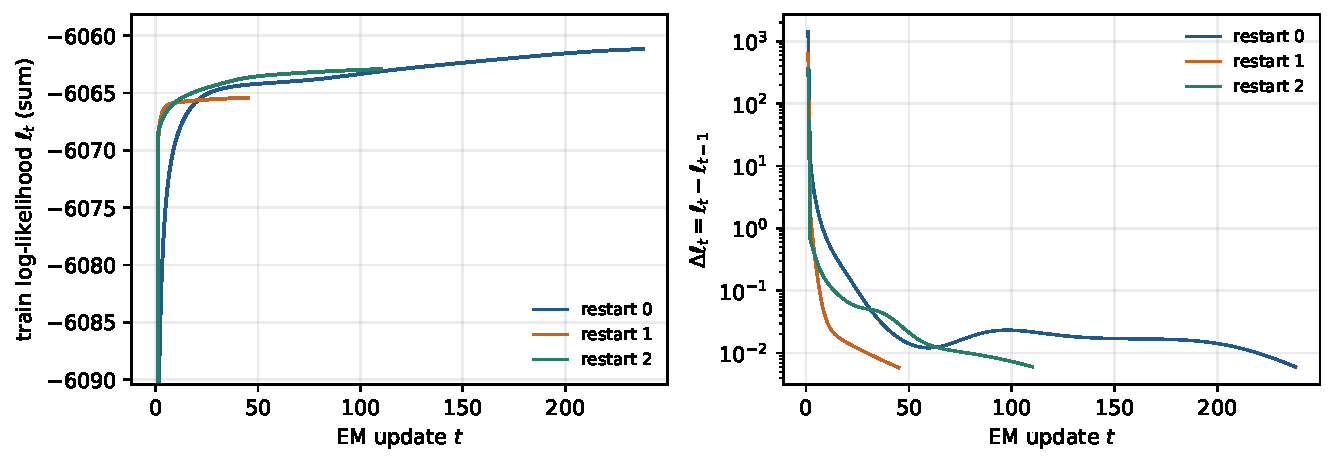
\includegraphics[width=\linewidth]{experiments/figures/em_curves.pdf}
\captionof{figure}{\seclink{sec:extension}{sec:exp-setup}{절의 $a=1$}, seed 0 조건에서 초기값을 달리한 세 EM 실행의 측정 결과.
왼쪽은 학습 데이터의 log-likelihood 합 $\ell_t$이다. 오른쪽은 $\Delta\ell_t$를 로그 축으로 나타낸 것이다. 세 실행 모두 $\Delta\ell_t\leq0$인 갱신은 없었다.
종료 시 $\ell$은 각각 $-6061.15$, $-6065.40$, $-6062.90$이다(갱신 횟수: 238, 45, 110).
단, 실제 global optimum은 알 수 없어 표시하지 않았다.}
\label{fig:initialization}
\end{center}
figure~\ref{fig:initialization}의 세 실행(파,주,초)은 모두 단조 증가 후 종료함을 보였지만, stop $\ell$은 최대 4.25 차이가 난다. 이 차이가 서로 다른 fixed point 때문인지, 단순히 살짝 평평한 likelihood에서 느리게 진행된 결과인지는 \seclink{sec:extension}{sec:conv-record}{절}에서도 구분하지 못했다.
변인 통제를 더 빡빡하게 하여 실험을 진행하면 종료 시 $\ell$이 바뀔 수 있다(\seclink{sec:extension}{sec:conv-record}{절, 종료 기준의 영향} 참조).
이에더해, component의 label 순서만 바꾸면 density는 같기에, 이를 서로 다른 local optimum으로
보아서는 안 된다. 여러 초기값에서 반복 실행하는 multiple restarts는 더 좋은 해를 찾을
가능성을 높이지만, 찾은 해가 전역 최적임을 보장하지는 않는다.

\subsection{Global Optimum의 보장 여부가 Anomaly Detection에 미치는 영향}
\label{sec:anomaly}
정상 데이터의 density를 GMM으로 추정하는 이상탐지 모델이 있다고 할 때,
학습된 parameter $\widehat\theta$로 식~\eqref{eq:loglik}의 혼합 density
$p_{\widehat\theta}(x)$를 계산하고, negative log-likelihood $-\log p_{\widehat\theta}(x)$를
anomaly score로 사용한다. 이 값이 threshold $\tau_a$보다 크면 이상으로 판정하며,
이는 density가 $c=e^{-\tau_a}$보다 낮은 점을 이상으로 보는 것과 같다.
정상 데이터의 true density $p_*$로 계산한 score와 비교하면, 두 score의 차이는
true density와 추정 density의 비율에 log를 취한 값이다.
따라서 density를 낮게 추정하면 anomaly score를 과대평가하고,
높게 추정하면 anomaly score를 과소평가한다.

False positive의 경우, 
추정된 해에서 드문 정상 cluster의 mixing coefficient가 너무 작거나 mean의 위치가 잘못되면,
해당 cluster에 속한 정상 샘플에서도 추정된 density가 낮아져 false positive가 발생할 수 있다.
이는 정상 사용자의 차단이나 불필요한 경보로 이어진다.

False negative의 경우,
서로 떨어진 정상 cluster들을 covariance가 큰 하나의 component로 추정하면,
관측값이 드문 cluster 사이에서도 density가 과대 추정될 수 있다.
그러면 이 영역의 이상 샘플을 정상으로 판정하는 false negative가 발생한다.

\begin{center}
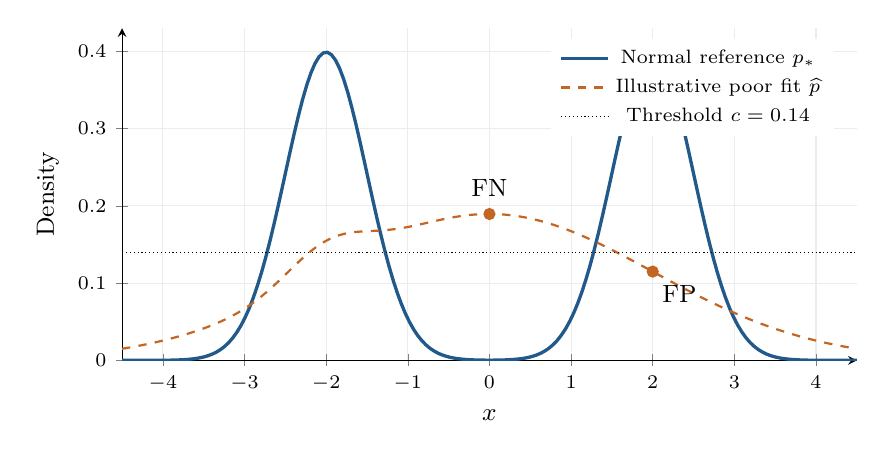
\begin{tikzpicture}
\begin{axis}[reportaxis,width=.9\linewidth,height=5.8cm,
 xmin=-4.5,xmax=4.5,ymin=0,ymax=.43,xlabel={$x$},ylabel={Density},
 legend pos=north east]
\addplot[mainblue,very thick,domain=-4.5:4.5,samples=180]
 {.5/(.5*sqrt(2*pi))*exp(-.5*((x+2)/.5)^2)
 +.5/(.5*sqrt(2*pi))*exp(-.5*((x-2)/.5)^2)};
\addlegendentry{Normal reference $p_*$}
\addplot[mainorange,dashed,thick,domain=-4.5:4.5,samples=180]
 {.95/(2*sqrt(2*pi))*exp(-.5*(x/2)^2)
 +.05/(.5*sqrt(2*pi))*exp(-.5*((x+2)/.5)^2)};
\addlegendentry{Illustrative poor fit $\widehat p$}
\addplot[black,densely dotted,domain=-4.5:4.5] {.14};
\addlegendentry{Threshold $c=0.14$}
\addplot[only marks,mark=*,mainorange] coordinates {(0,.18950) (2,.11494)};
\node[font=\small,anchor=south] at (axis cs:0,.20) {FN};
\node[font=\small,anchor=north west] at (axis cs:2,.11) {FP};
\end{axis}
\end{tikzpicture}
\captionof{figure}{density 추정 오차에 따른 false positive과 false negative.
$p_*=\tfrac12\Normal(-2,0.5^2)+\tfrac12\Normal(2,0.5^2)$,
$\widehat p=0.95\Normal(0,2^2)+0.05\Normal(-2,0.5^2)$로 구성한 예이다.
$\widehat p$가 실제 EM의 local optimum인지는 확인하지 않았다.}
\label{fig:anomaly}
\end{center}
figure~\ref{fig:anomaly}에서 $x=0$은 $p_*(0)\approx0.00027<c$이지만
$\widehat p(0)\approx0.1895>c$이기에 density가 낮은 이상점을 정상으로 판정한다.
반대로 정상 mode의 중심 $x=2$는 $p_*(2)\approx0.3989>c$이지만
$\widehat p(2)\approx0.1149<c$이기에 false positive로 된다.
이 예는 threshold를 고정했을 때 density 추정 오차가 판정에 미치는 영향을 보여 준다.
또한 $\widehat p(0)>\widehat p(2)$이기에 이상점 0의 anomaly score가 정상점 2보다 낮다.
따라서 하나의 density threshold로 두 점을 모두 올바르게 분류할 수 없다.
검증 데이터로 threshold를 조정해 false positive를 보정하더라도 이러한 순위 역전은 해결되지 않는다.
평가 샘플에서 순위 역전이 발생하면 AUROC나 PR-AUC도 낮아질 수 있으며,
감소 폭은 전체 정상/이상 샘플의 score 분포에 따라 달라진다.

초기값에 따라 $\widehat p$가 달라지면 같은 샘플에 대한 탐지 결과도 달라질 수 있다.
학습 데이터에 이상 샘플이 섞여 있고 특정 component가 그 샘플에 집중되면,
이상 샘플의 density를 높게 추정할 수도 있다. 따라서 학습 데이터의 likelihood가 높아진다고
탐지 성능까지 좋아지는 것은 아니다.
이를 완화하려면 multiple restarts와 covariance 제약을 사용하고,
정상 검증 데이터로 threshold를 조정할 수 있다. label이 있다면 precision--recall과
목표 false-positive rate에서의 recall도 평가해야 한다.
학습 데이터의 global MLE를 구하더라도 데이터 오염, model misspecification,
distribution shift의 영향은 별도로 확인해야 한다.


\section{GMM 파라미터 추정의 EM 대안}

\subsection{Parametric denoising score matching}
\label{sec:dsm}

강의를 들을 때, GMM의 training algorithm으로 flow matching을 충분히 사용할 수 있을 것 같다는 생각이 들었다. gaussian mixture과 score matching 키워드로 검색해보니 관련한 연구들이 있었으며, 내가 생각했던 것과 비슷한 흐름으로 진행한 연구가 있어 가져왔다.
\citet{score2025}은 이론적으로 parameter recovery가 불가능한 조건에서도 고려할 수 있는 방법론으로, score를 학습해 목표 분포에 가까운 샘플을 생성하는 sampler를 구성하는 방식을 제안하였다.
하지만, 과제는 parameter 추정을 요구하기에, GMM의 analytic score를 DSM objective에 대입해 $\pi,\mu,\Sigma$를 직접 다루는 방식을 구상해보았다.

전체 흐름은 일반적인 flow matching과 유사하다. score $\nabla_x\log p(x)$는 입력 $x$에 대한 log-density의 gradient이며, 원본 데이터 $x_0$에 noise를 더해 $x_t=a_tx_0+b_t\epsilon$을 만들고, $\epsilon\sim\Normal(0,I_d)$, $a_t=e^{-t}$, $b_t=\sqrt{1-e^{-2t}}$이며 $t>0$은 noise level이다.
변환된 모델도 mean이 $a_t\mu_k$, covariance가 $C_{k,t}=a_t^2\Sigma_k+b_t^2I_d$인 GMM이기에,
그 score를 정확히 계산할 수 있다.
\begin{equation}
 s_{\theta,t}(x)=\sum_{k=1}^{K}r_{k,t}(x)\,C_{k,t}^{-1}(a_t\mu_k-x)
 \label{eq:gmm-score}
\end{equation}
$r_{k,t}(x)$는 noise가 포함된 GMM에서 식~\eqref{eq:estep}로 계산한 responsibility이다.
이 score를 다음 denoising loss에 대입한다.
\begin{equation}
 \mathcal L_{\mathrm{DSM}}(\theta)
 =\E_{t,\,x_0,\,\epsilon}\left[\,b_t^2\left\|
 s_{\theta,t}(a_tx_0+b_t\epsilon)+\frac{\epsilon}{b_t}\right\|_2^2\,\right]
 \label{eq:parametric-dsm}
\end{equation}
noise로부터 계산한 $-\epsilon/b_t$를 regression target으로 삼으며,
이 손실은 true score에 대한 mse와 $\theta$에 무관한 상수만큼만 다르다~\citep{vincent2011}.
true density를 몰라도 샘플만으로 학습할 수 있다는 엄청난 아이디어이다.
여러 $t$를 사용하면 서로 다른 레벨의 분포를 학습하며, 가중치 $b_t^2$는 작은 $t$에서 target이 커지는 영향을 보정한다.

logit $u_k$, mean $\mu_k$, lower triangular matrix $L_k$를 학습하고,
$\pi=\softmax(u)$, $\Sigma_k=L_kL_k^\top+\lambda_0I_d$ ($\lambda_0>0$)로 변환한다.
$L_k$의 대각 성분에는 softplus를 적용해 유효한 covariance를 구성한다.
학습 후 얻는 $\widehat\Sigma_k$는 원래 데이터의 covariance이며, noise가 포함된 $C_{k,t}$와 구별된다.
추정된 GMM으로 density를 직접 계산할 수 있고, \secref{sec:extension}{절에서} EM과의 실험 결과를 비교한다.

\begin{center}
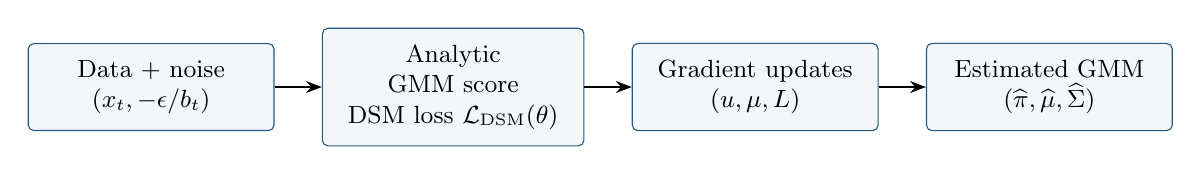
\begin{tikzpicture}[node distance=6mm]
\node[box,text width=2.7cm] (data) {Data + noise\\$(x_t,-\epsilon/b_t)$};
\node[box,text width=2.9cm,right=of data] (score) {Analytic GMM score\\DSM loss $\mathcal L_{\mathrm{DSM}}(\theta)$};
\node[box,text width=2.7cm,right=of score] (opt) {Gradient updates\\$(u,\mu,L)$};
\node[box,text width=2.7cm,right=of opt] (out) {Estimated GMM\\$(\widehat\pi,\widehat\mu,\widehat\Sigma)$};
\draw[arrow] (data)--(score);
\draw[arrow] (score)--(opt);
\draw[arrow] (opt)--(out);
\end{tikzpicture}
\captionof{figure}{Parametric DSM의 estimation 절차. GMM의 analytic score로 손실을 계산하고
parameter를 직접 갱신한다.}
\label{fig:dsm}
\end{center}

\subsection{TGMM}
\label{sec:tgmm}
\citet{tgmm2026}은
합성 GMM 데이터셋으로 Transformer estimator를 meta-training한 뒤,
새 데이터셋의 parameter를 한 번의 forward pass로 예측한다.
논문에서 제안한 기본 모델은 $\Sigma_k=I_d$로 고정한다. covariance를 고정하지 않고 추정하게 되면, 차원이 커질수록 EM알고리즘에 비해 TGMM의 log-likelihood성능이 급격하게 떨어지는 문제를 보인다고 한다. 다만, 과제는 공분산 추정까지도 요구하였기에, 원 논문의 Appendix H.1, covariance 추정을 포함한 방법을 위주로 공부하였다.

label이 없는 새 데이터셋 $X$와 사용자가 지정한 component 수 $K$를 입력한다.
각 샘플을 token으로 변환하고 $K$의 embedding을 붙인 뒤, 공통 Transformer와 $K$별 readout으로 parameter를 출력한다.
\begin{equation}
 (\widehat\pi,\widehat\mu,\widehat\sigma)
 =\operatorname{Readout}_{K}\!\left(
 \operatorname{TF}_{\Phi}\!\left(
 \operatorname{Readin}\bigl([X\,\|\,\operatorname{embed}(K)]\bigr)\right)\right),
 \qquad \widehat\Sigma_k=\diag(\widehat\sigma_k^2)
 \label{eq:tgmm}
\end{equation}
readin은 입력을 공통 hidden representation으로 변환하고,
readout은 attentive pooling으로 샘플의 표현을 $K$개의 component별 표현으로 모은다.
$\Phi$는 전체 network의 학습 parameter로, 각 데이터셋의 GMM parameter $\theta$와 구별된다.
mixing coefficient의 합이 1이고 scale이 양수가 되도록 출력 변환을 적용할 수 있다.
예를 들어 mixing coefficient에는 softmax, scale에는 softplus와 작은 양수를 사용할 수 있으며,
이는 원 논문의 activation을 재현한 것이 아니라 출력 제약을 구체화한 예이다.

\begin{center}
\begin{minipage}{\linewidth}
\centering
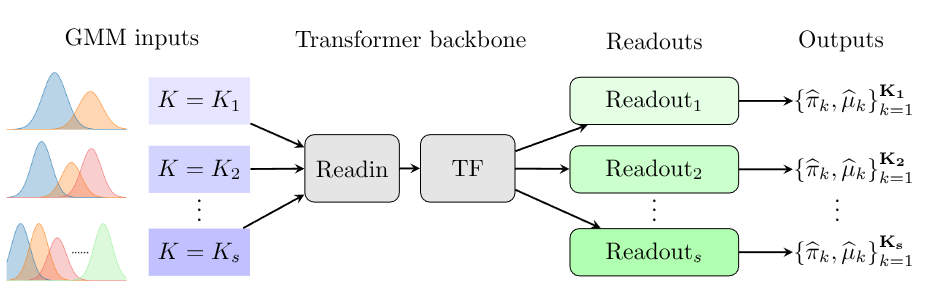
\includegraphics[width=\linewidth]{tgmm_figure1.png}
\captionof{figure}{논문의 Figure 1, TGMM의 기본 구조. 여러 component 수 $K$에 대해 Transformer backbone을 공유하고 $K$별 readout으로 mixing coefficient와 mean을 예측한다. covariance는 사전 고정되어, output에 나오지 않는다~\citep{tgmm2026}.}
\label{fig:tgmm-architecture}
\end{minipage}
\end{center}

true parameter를 아는 합성 데이터셋에서, mean의 squared loss와 mixing coefficient의
cross-entropy를 minimize하며, H.1에서는 scale $\sigma_k$의 mean-square loss를 추가한다.
각 scale 원소를 제곱한 값이 covariance의 대각 성분이기에 비대각 상관관계(원문 Off-diagonal elements, 는 추정하지 않는다.
논문의 평가에서는 mean의 제곱거리로 component 순서를 맞춘 뒤 다른 parameter에도 같은 대응을 적용한다.
학습 후에는 $\Phi$를 고정하고 새 데이터셋에 식~\eqref{eq:tgmm}를 적용한다.
따라서 추론할 데이터셋에는 label이 필요 없지만,
meta-training에는 합성 데이터의 참 parameter를 supervision으로 사용한다.

\begin{center}
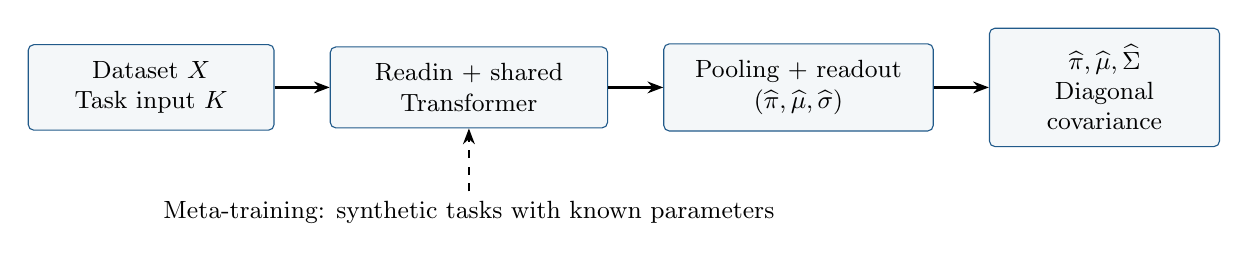
\begin{tikzpicture}[node distance=7mm]
\node[box,text width=2.7cm] (input) {Dataset $X$\\Task input $K$};
\node[box,text width=3.1cm,right=of input] (tf) {Readin + shared\\Transformer};
\node[box,text width=3cm,right=of tf] (out) {Pooling + readout\\$(\widehat\pi,\widehat\mu,\widehat\sigma)$};
\node[box,text width=2.5cm,right=of out] (params) {$\widehat\pi,\widehat\mu,\widehat\Sigma$\\Diagonal covariance};
\draw[arrow] (input)--(tf);
\draw[arrow] (tf)--(out);
\draw[arrow] (out)--(params);
\node[font=\small,align=center,below=8mm of tf] (train)
 {Meta-training: synthetic tasks with known parameters};
\draw[arrow,dashed] (train)--(tf);
\end{tikzpicture}
\captionof{figure}{TGMM의 estimation 절차. pre-train한 network로 새 데이터셋의 parameter를 예측하며,
covariance는 원 논문 H.1의 diagonal 방식으로 추정한다.}
\label{fig:tgmm}
\end{center}

\subsection{두 추정법과 EM의 비교}
\begin{center}\begin{minipage}{\linewidth}\centering
\captionof{table}{EM과 두 대안의 비교. DSM은 analytic GMM score로 parameter를 직접 추정하는 방식,
TGMM은 원 논문 H.1의 covariance 추정을 포함한 방식이다.}
\label{tab:comparison}
\small
\setlength{\tabcolsep}{4pt}
\renewcommand{\arraystretch}{1.15}
\begin{tabularx}{\linewidth}{@{}>{\raggedright\arraybackslash}p{1.55cm}YYY@{}}
\toprule
비교 항목 & EM & Parametric DSM & TGMM \\
\midrule
핵심 아이디어 &
responsibility와 가중 통계량을 반복 계산해 log-likelihood를 높인다. &
여러 noise level의 denoising loss를 gradient로 최소화한다. &
합성 데이터셋으로 estimator를 학습한 뒤 새 데이터셋에 재사용한다. \\
\addlinespace
파라미터 산출 &
responsibility의 합으로 $\pi$를, weighed sum/covariance로 $\mu,\Sigma$를 구한다. &
$\pi=\softmax(u)$, mean 직접 학습, $\Sigma=LL^\top+\lambda_0I$로 full covariance를 구한다. &
readout으로 $\pi,\mu,\sigma$를 출력하고 $\Sigma=\diag(\sigma^2)$로 구한다. \\
\addlinespace
장점 &
closed-form 갱신이 간단하며 정확한 EM은 likelihood 비감소를 보장한다. &
closed-form M-step 없이 mini-batch 학습이 가능하고, 여러 평활화 수준을 활용한다. &
pre-train 후 한 번의 forward pass로 추정하며, 학습에서 다룬 여러 $K$에 backbone을 공유한다. \\
\addlinespace
한계 &
초기값 및 local minimum에 민감하고, covariance의 퇴화를 막는 제약이 필요하다. &
non-convex optimization으로, 초기값 및 noise 설정에 민감하다. likelihood 비감소와 전역 최적해를 보장하지 않으며 추가 계산이 든다. &
pretrain 비용과 학습 분포에 대한 의존성이 있다. 또한, 애초에 이 논문은 EM과의 비교 뿐만이 아닌, 모멘트 기반 스펙터럴 알고리즘과의 비교까지 본 것으로, 비대각 공분산까지 추정의 한계가 존재하며, 학습 성공 및 global MLE를 보장하지 않는다. \\
\bottomrule
\end{tabularx}
\end{minipage}\end{center}

두 대안이 항상 EM보다 좋은 해를 찾는 것은 아니다.
DSM은 component가 멀리 떨어진 mixture에서 mixing coefficient 복원이 어려울 수 있고,
정규성 조건 아래에서는 MLE보다 통계 효율이 낮을 수 있다~\citep{koehler2023}.
이는 실제 EM의 local minimum나 유한 샘플 성능과는 별개의 비교이며,
\secref{sec:extension}{절 실험}에서도 DSM의 일관된 정확도, 속도 우위는 없었다.
TGMM의 원 논문은 일부 조건에서 EM보다 작은 parameter 오차를 보고하지만,
고차원에서는 likelihood가 baseline보다 낮았다.
Transformer가 EM을 근사할 수 있다는 이론도 meta-training의 성공이나 전역 최적해를 보장하지 않는다.

이상탐지에서는 두 방법 모두 추정 density의 $-\log p_{\widehat\theta}(x)$를 사용한다.
이는 vector인 score $\nabla_x\log p(x)$와 다르며,
score는 mode 사이의 local minimum에서도 0일 수 있어 그 크기만으로 이상 여부를 판단하기 어렵다.
parameter 오차나 분포 근사 오차가 작아도 tail 영역의 density가 정확하다는 보장은 없기에, 탐지 성능은 별도로 평가하는 것이 필요하다.

\section{EM과 Parametric DSM 실험 비교}
\label{sec:extension}
\phantomsection\label{sec:exp-setup}%
EM과 Parametric DSM을 직접 실행한 결과를 비교해보았다. TGMM 실험의 경우에는 수식의 복잡성과 llm의 구현에 대한 검증에 적지 않은 시간을 투자해야할 것 같다고 판단하여 수행하지 않았다.
$d=2$, $K=3$인 GMM에서 mixing coefficient를 $(0.5,0.3,0.2)$,
mean을 $-ae_1,0,ae_1$로 두고, component가 겹치는 $a=1$과 분리된 $a=4$를 비교하였다.
두 방법 모두 같은 데이터(train/val/test: $2000/1000/10000$)와 초기값에서 full covariance를 추정한다.
seed 5개에서 각각 3회 진행하였으며, EM은 log-likelihood의 상대 증가량 $10^{-6}$을 기준으로 종료하고,
DSM은 여러 noise level을 사용해 5000회 갱신하였다.
모델은 validation NLL로 선택하되, EM은 restart별 최종 모델 3개,
DSM은 중간 checkpoint를 포함한 30개를 후보로 삼았다.
실험 코드 및 설정 등은 \href{https://github.com/ga111o/EM-algorithm-and-GMM-parameter-estimation}{GitHub}에 위치한다.

$E_\pi$, $E_\mu$, $E_\Sigma$는 true component와 estimated component의 순서를 대응시킨 뒤 계산한
각 parameter 원소의 RMSE이며, Test NLL은 평가 샘플의 평균 $-\log p_{\widehat\theta}(x)$일때, 
\begin{center}\begin{minipage}{\linewidth}\centering
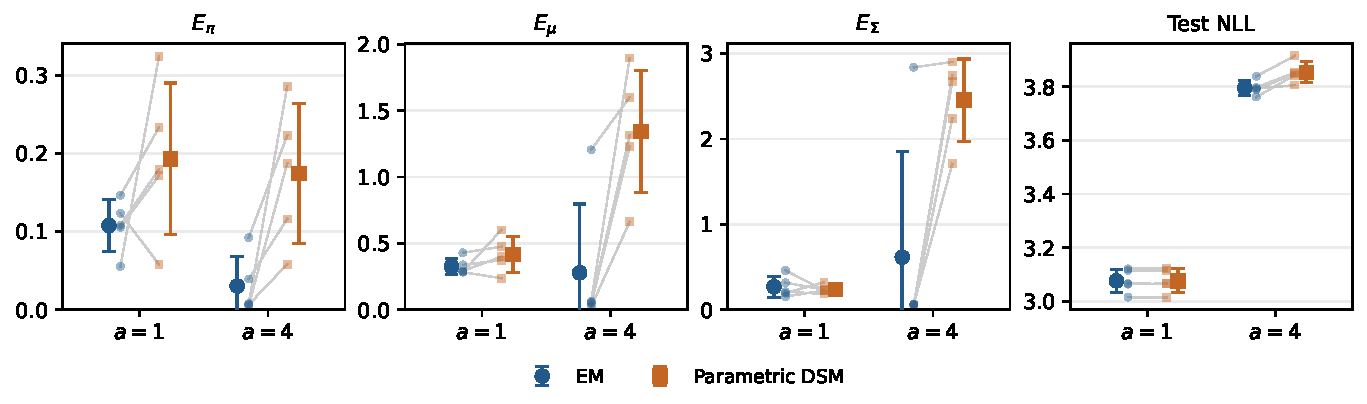
\includegraphics[width=\linewidth]{experiments/figures/main_comparison.pdf}
\captionof{figure}{component 분리에 따른 EM과 Parametric DSM의 비교.
원(EM)과 사각형(DSM)의 오차 막대는 seed 5개에 대한 평균 $\pm$ 샘플의 sd이고,
연한 점은 5개는 각 seed에서 validation NLL로 선택한 모델의 값이다.
parameter 오차의 축은 0에서 시작한다.}
\label{fig:main}
\end{minipage}\end{center}

$a=1$에서, 즉, component가 겹치는 조건에서는 평균 test NLL은 두 방법 모두 약 3.076이었다.
같은 seed끼리 비교한 NLL 차이(DSM$-$EM)도 평균 약 $3\times10^{-4}$로 작았고,
어느 방법이 낮은지는 seed에 따라 달랐다.
반면 parameter 오차에서는 $E_\pi$와 $E_\mu$는 EM이, $E_\Sigma$는 DSM이 평균적으로 낮았다.
따라서 이 조건에서 DSM의 density 적합도는 EM과 비슷했지만,
mixing coefficient와 mean의 복원까지 더 정확해진 것은 아닌 것을 알 수 있다.

figure~\ref{fig:measured-density}는 figure~\ref{fig:initialization}의 $a=1$, seed 0에서
학습 데이터의 종료 $\ell$이 가장 높은 EM 실행과 가장 낮은 실행을 true density와 비교한 것이다.
\begin{center}\begin{minipage}{\linewidth}\centering
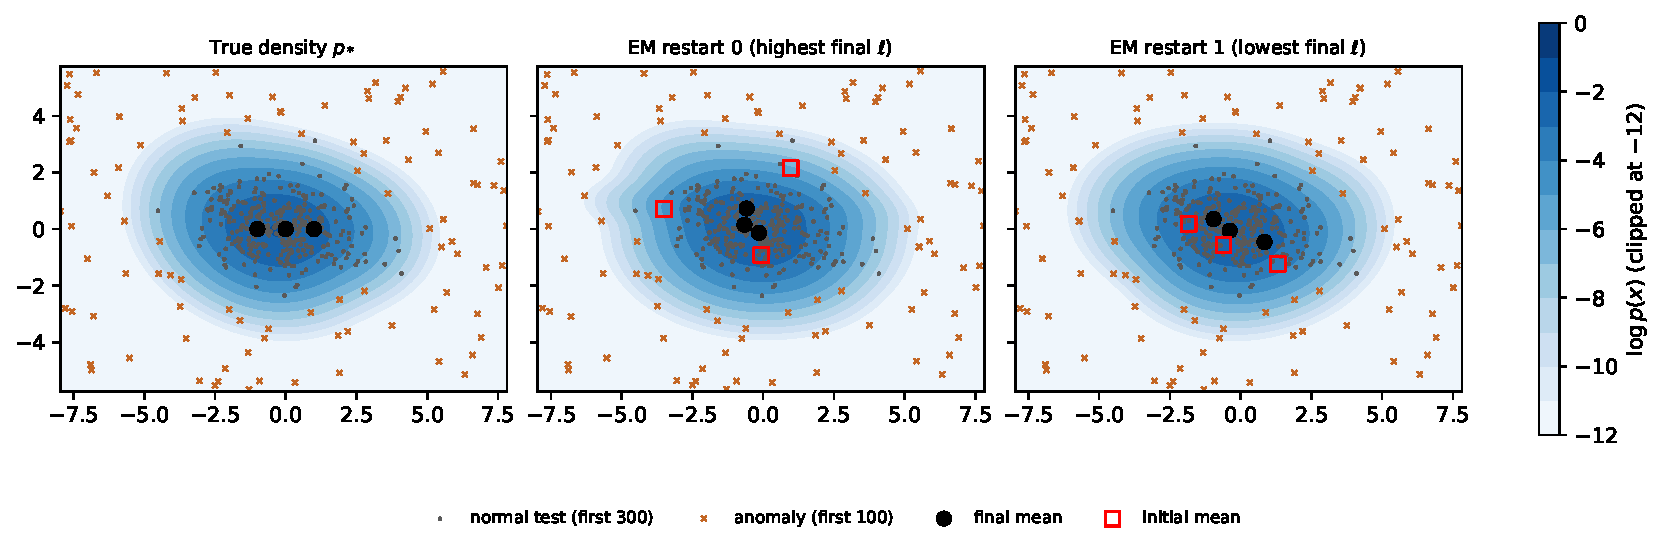
\includegraphics[width=\linewidth]{experiments/figures/density.pdf}
\captionof{figure}{$a=1$, seed 0에서의 true density와 EM으로 추정한 density.
종료 $\ell$이 가장 높은 restart 0과 가장 낮은 restart 1을 같은 좌표 범위와 $\log p$ 등고선 기준 비교.
회색 점과 주황색 x는 정상 및 이상 샘플 각각 300개와 100개를 표시한다.
검은 원은 true mean 또는 최종 추정 mean이며, 빨간 ㅁ은 초기 mean이다.}
\label{fig:measured-density}
\end{minipage}\end{center}

두 실행은 추정 mean의 위치가 다르지만, 정상 샘플이 모인 중심부의 density 윤곽은 true 분포와 비슷하다.
component 순서를 대응시킨 뒤에도 두 실행의 parameter 원소 차이는 최대 0.99였으며,
평가 샘플에서 두 추정 density의 log 값 차이의 절댓값 평균은 0.057이었다.
component가 겹치는 경우, 각각의 component를 다르게 배치해도 전체 mixture density는 비슷하게 설명할 수 있음을 알 수 있다.
시각화 결과가 비슷하다는 것으로 true parameter가 정확히 복원되었다고는 할 수 없다.

이에 더해, 또한 종료 $\ell$이 낮은 restart 1의 validation NLL이 오히려 더 낮아
(3.0047 대 3.0071) 최종 모델로 선택되었다.
즉, 이 실험에서는 학습 데이터에 더 잘 맞는 실행이 검증 데이터에서도 더 좋은 것은 아니었다.
figure~\ref{fig:anomaly}의 예시처럼 정상 cluster을 놓치는 현상은 보이지 않았고,
두 실행의 seed 0 AUROC도 모두 약 0.99956으로 가까웠다.
초기값에 따른 parameter 차이가 바로 탐지 성능 차이로 이어지지는 않음을 보였다.

$a=4$에서, 즉, component가 분리되었을 때에는 평균 test NLL은 EM이 3.796, DSM이 3.853이었고, 다섯 seed 모두 EM이 더 낮았다.
세 parameter 오차도 평균적으로 EM이 작았으며, 특히 $E_\mu$는 0.278 대 1.343,
$E_\Sigma$는 0.614 대 2.452로 차이가 났다.
$a=1$과 달리 이 조건에서는 주어진 학습 횟수 내에서 density 적합도와 parameter 복원 모두 EM이 앞섰다.

다만 EM의 큰 표준편차도 함께 보는 것이 필요하다.
seed 0의 선택 모델은 $E_\mu\approx1.21$, $E_\Sigma\approx2.84$였지만,
나머지 네 seed에서는 각각 0.064와 0.066 미만이었다.
즉, EM의 평균 오차는 특정 seed에서, 추정이 잘 되지 않은 결과에 크게 영향을 받은 것을 알 수 있다.
component를 분리했을 때 대체로 복원이 좋아졌어도, 모든 실행에서 안정적으로 좋은 결과를 얻은 것은 아니다.

\phantomsection\label{sec:conv-record}%
이 편차를 바로 local minima의 차이로 해석하기는 어렵다.
실제로, $a=4$, seed 0의 두 EM restart는 종료 허용오차를 $10^{-10}$으로 낮추고 반복을 계속하였을 때, $\ell$이 약 138 높아졌다. 즉, 느리게 개선되는 구간에서 일찍 멈춘 영향일 수 있다.
DSM 역시 $a=4$의 마지막 500회 갱신에서 15개 실행 중 13개의 validation NLL이 감소하였다.
즉, 실험 세팅에 따라 결과가 달라질 수 있다.

시간은 실행당 EM이 0.09--1.63초, DSM이 5.56--5.77초였다(val 계산 포함).
이 설정에서 DSM은 더 긴 실행 시간과 더 많은 모델 선택 후보를 사용했지만,
$a=1$에서는 NLL이 비슷했고 $a=4$에서는 오차가 더 컸다.
즉, 이번 구현 및 설정에서는 추가 사용하는 컴퓨팅 자원에 상응하는 정확도 개선을 확인하지 못했다.

정상 데이터로 학습한 모델의 $-\log p_{\widehat\theta}(x)$를 anomaly score로 사용하고,
정상 검증 score의 95백분위수를 threshold로 정하며,
정상 검증 데이터의 참 density 분포에서 1백분위수보다 density가 낮은 인공 이상 샘플 1000개를
정상 평가 샘플 10000개와 함께 평가하였다.
이때, 이상탐지 결과를 비교하면 아래와 같다.
\begin{center}\begin{minipage}{\linewidth}\centering
\captionof{table}{Validation NLL로 선택한 모델의 이상탐지 성능.
seed 5개에 대한 평균 $\pm$ 샘플 표준편차이다. FPR은 낮을수록, 나머지 지표는 높을수록 좋다.}
\label{tab:detection}
\small
\setlength{\tabcolsep}{3pt}
\begin{tabular}{@{}llccccc@{}}
\toprule
Condition & Method & FPR & Recall & Precision & AUROC & PR-AUC \\
\midrule
% Selected-model rows from tab_detection.tex, restricted to a=1 and a=4.
$a=1$ & EM & $0.050\pm0.002$ & $1.000\pm0.000$ & $0.667\pm0.007$ & $0.9994\pm0.0001$ & $0.9942\pm0.0009$ \\
$a=1$ & DSM & $0.049\pm0.003$ & $1.000\pm0.000$ & $0.670\pm0.012$ & $0.9994\pm0.0001$ & $0.9942\pm0.0008$ \\
\addlinespace
$a=4$ & EM & $0.054\pm0.004$ & $1.000\pm0.000$ & $0.648\pm0.015$ & $0.9993\pm0.0001$ & $0.9926\pm0.0012$ \\
$a=4$ & DSM & $0.054\pm0.005$ & $0.999\pm0.001$ & $0.649\pm0.023$ & $0.9985\pm0.0002$ & $0.9857\pm0.0015$ \\
\bottomrule
\end{tabular}
\end{minipage}\end{center}

표~\ref{tab:detection}에서 두 방법 모두 평균 recall이 0.999 이상으로,
선택한 threshold에서는 이상 샘플을 거의 모두 탐지하였다.
FPR은 약 0.05로 비슷했지만 precision은 약 0.65--0.67이었다.
정상 샘플이 이상 샘플의 10배이므로, 정상의 약 5\%를 false positive로 보이면 약 500개의 false positive가 생기기 때문이다.
높은 recall이나 AUROC가 곧 높은 precision을 뜻하지는 않으며, threshold와 정상/이상 비율도 함께 보아야 한다.

$a=1$에서는 AUROC와 PR-AUC도 두 방법이 거의 같았다.
반면 $a=4$에서는 DSM의 AUROC와 PR-AUC가 모두 낮아,
현재 threshold의 탐지율이 비슷해도 score의 순위 구분 능력에는 차이가 나타났다.
다만 이상 샘플을 true density가 낮은 영역에서 골랐기에 애초에 탐지가 쉬운 조건이다.
figure~\ref{fig:measured-density}의 초기값별 비교와 마찬가지로,
이러한 높은 탐지율만으로 parameter 추정 오차나 초기값의 영향이 일반적으로 작다고 결론 내리기는 어렵다.

원본 논문의 결과만 보았을 때에는, Parametric DSM이 대부분의 상황에서 좋을 것으로 예상했다. 다만, 실제 실험 결과,
Parametric DSM은 component가 겹치는 조건에서 EM과 비슷한 density 적합도를 얻었지만,
parameter 복원이나 실행 시간에서 일관된 이점은 보이지 않았다.
component가 분리된 조건에서는 현재 계산량과 종료 기준 아래에서 EM의 추정 결과가 더 좋았다.

\section*{Acknowledgement}
GMM과 EM을 공부할 때, 교수님의 교안과 함께 \href{https://blog.google/innovation-and-ai/models-and-research/gemini-models/3-8-flash-and-3-8-flash-cyber/}{Gemini 3.8 Flash (Extended)}를 사용하였으며, 추가 실험 설계에 \href{https://openai.com/index/introducing-gpt-6-1-sol/}{OpenAI GPT 6.1 Sol (xhigh)}를 사용하였습니다. 또한, 본 보고서의 주요 수식 및 latex 문법 작성에 \href{https://www.anthropic.com/claude-opus-5-5}{Claude Opus 5.5 (medium)}를 사용하였으며, 본 보고서의 본문을 작성할 때 \href{https://cursor.com/help/ai-features/tab}{Cursor}의 코드 자동완성 기능을 사용하였음을 밝힙니다.
보고서의 최종 내용은 작성자의 이해와 판단, 수정을 거쳐 나왔음을 밝힙니다.


\begingroup
\small
\setlength{\parskip}{2pt}
\begin{thebibliography}{9}

\bibitem[Chen et al.(2025)]{score2025}
Chen, S., Kontonis, V., \& Shah, K. (2025).
Learning general Gaussian mixtures with efficient score matching.
In N. Haghtalab \& A. Moitra (Eds.),
\textit{Proceedings of the thirty-eighth conference on learning theory}
(Vol.~291, pp.~1029--1090). PMLR.
\url{https://proceedings.mlr.press/v291/chen25e.html}

\bibitem[Chen et al.(2026)]{tgmm2026}
Chen, Z., Wu, R., \& Fang, G. (2026).
\textit{Transformers as unsupervised learning algorithms: A study on Gaussian mixtures}.
arXiv.
\url{https://arxiv.org/abs/2505.11918v2}

\bibitem[Dempster et al.(1977)]{dempster1977}
Dempster, A.~P., Laird, N.~M., \& Rubin, D.~B. (1977).
Maximum likelihood from incomplete data via the EM algorithm.
\textit{Journal of the Royal Statistical Society: Series B (Methodological), 39}(1), 1--22.
\url{https://doi.org/10.1111/j.2517-6161.1977.tb01600.x}

\bibitem[Jin et al.(2016)]{jin2016}
Jin, C., Zhang, Y., Balakrishnan, S., Wainwright, M.~J., \& Jordan, M.~I. (2016).
Local maxima in the likelihood of Gaussian mixture models: Structural results and algorithmic consequences.
In D.~D. Lee, M. Sugiyama, U. von Luxburg, I. Guyon, \& R. Garnett (Eds.),
\textit{Advances in neural information processing systems}
(Vol.~29, pp.~4116--4124). Curran Associates.
\url{https://proceedings.neurips.cc/paper/2016/hash/3875115bacc48cca24ac51ee4b0e7975-Abstract.html}

\bibitem[Koehler et al.(2023)]{koehler2023}
Koehler, F., Heckett, A., \& Risteski, A. (2023).
Statistical efficiency of score matching: The view from isoperimetry.
In \textit{International Conference on Learning Representations}.
\url{https://openreview.net/forum?id=TD7AnQjNzR6}

\bibitem[Vincent(2011)]{vincent2011}
Vincent, P. (2011).
A connection between score matching and denoising autoencoders.
\textit{Neural Computation, 23}(7), 1661--1674.
\url{https://doi.org/10.1162/NECO_a_00142}

\bibitem[Wu(1983)]{wu1983}
Wu, C.~F.~J. (1983).
On the convergence properties of the EM algorithm.
\textit{The Annals of Statistics, 11}(1), 95--103.
\url{https://doi.org/10.1214/aos/1176346060}

\end{thebibliography}
\endgroup
\end{document}
